\documentclass{svmult}
\usepackage{graphicx}
\usepackage{amsmath}
\begin{document}
\title{ SAAS: A Tool for Satisfiability analysis of 
		Assertion Specifications}

\maketitle
\thispagestyle{empty}

\abstract
{
Software Verification has become a must necessary step of Software engineering.
For performing software verification we need to have a well written requirement 
Specification. Generally requirements are written in Natural Language processing
which can be ambiguous or may have contradictory requirements. If a code is verified 
against this erroneous specification it cannot result to a correct software output.
In this paper we want to present a tool ToYicesTranslator  that can check if the 
requirements are inconsistent or unsatisfiable.This tool consists of 3 parts, First 
our input file is given to a parser,it will generate a symbol table and a syntax tree.
Now using this symbol table and syntax tree ToYicesTranslator will generate a file 
which is compatible with Yices.Yices is tool for checking satisfiability of the given 
expression.If Yices gives SAT as result then the given specifications is satisfiable 
and consistent.
}


\section{Introduction}

Software verification has become a necessary step of Software engineering.
It assures that the developed software fully satisfies its requirements. 
If a software undergoes verification successfully then it can be said
that the software is bug free and will work correctly.

we want to perform software verification to get error free, bug free
code, so that after delivery there occur no problem.To perform Software 
verification successfully one need to have correct requirement specification 
as in software verification the software is verified against the requirement 
specification. If the requirements are not stated properly and correctly then 
if the software passes verification, we cannot get bug free code. So it is 
necessary to have the specification correct.

Now, as the specifications are written in Natural Language processing,
there may be ambiguity, contradiction which are not easily visible. But 
the presence of ambiguous or contradictory statements will make the 
specification buggy. we developed a tool that will help us to  check whether
the specification is contradictory using Yices which is  a satisfiability
modulo theory solver that will check whether the given assertions are 
correct or not.  




\section{CheckSpec: Major Building Blocks} \label{sec4}


\noindent
{\bf Parser: Lex AND Yacc} 
Lex is an unix utility that parses the input file of characters.It uses 
regular expression matching to tokenize the contents of the file.Rules 
for the tokens are written in the lex file. Matching the patterns of the 
rules lex generate tokens.Each rule specified in the lex has an associated
action.Typically this action returns a token which represents the matching string 
for subsequent use by the parser.The following represents a lex pattern and action:

\begin{figure}[!h]
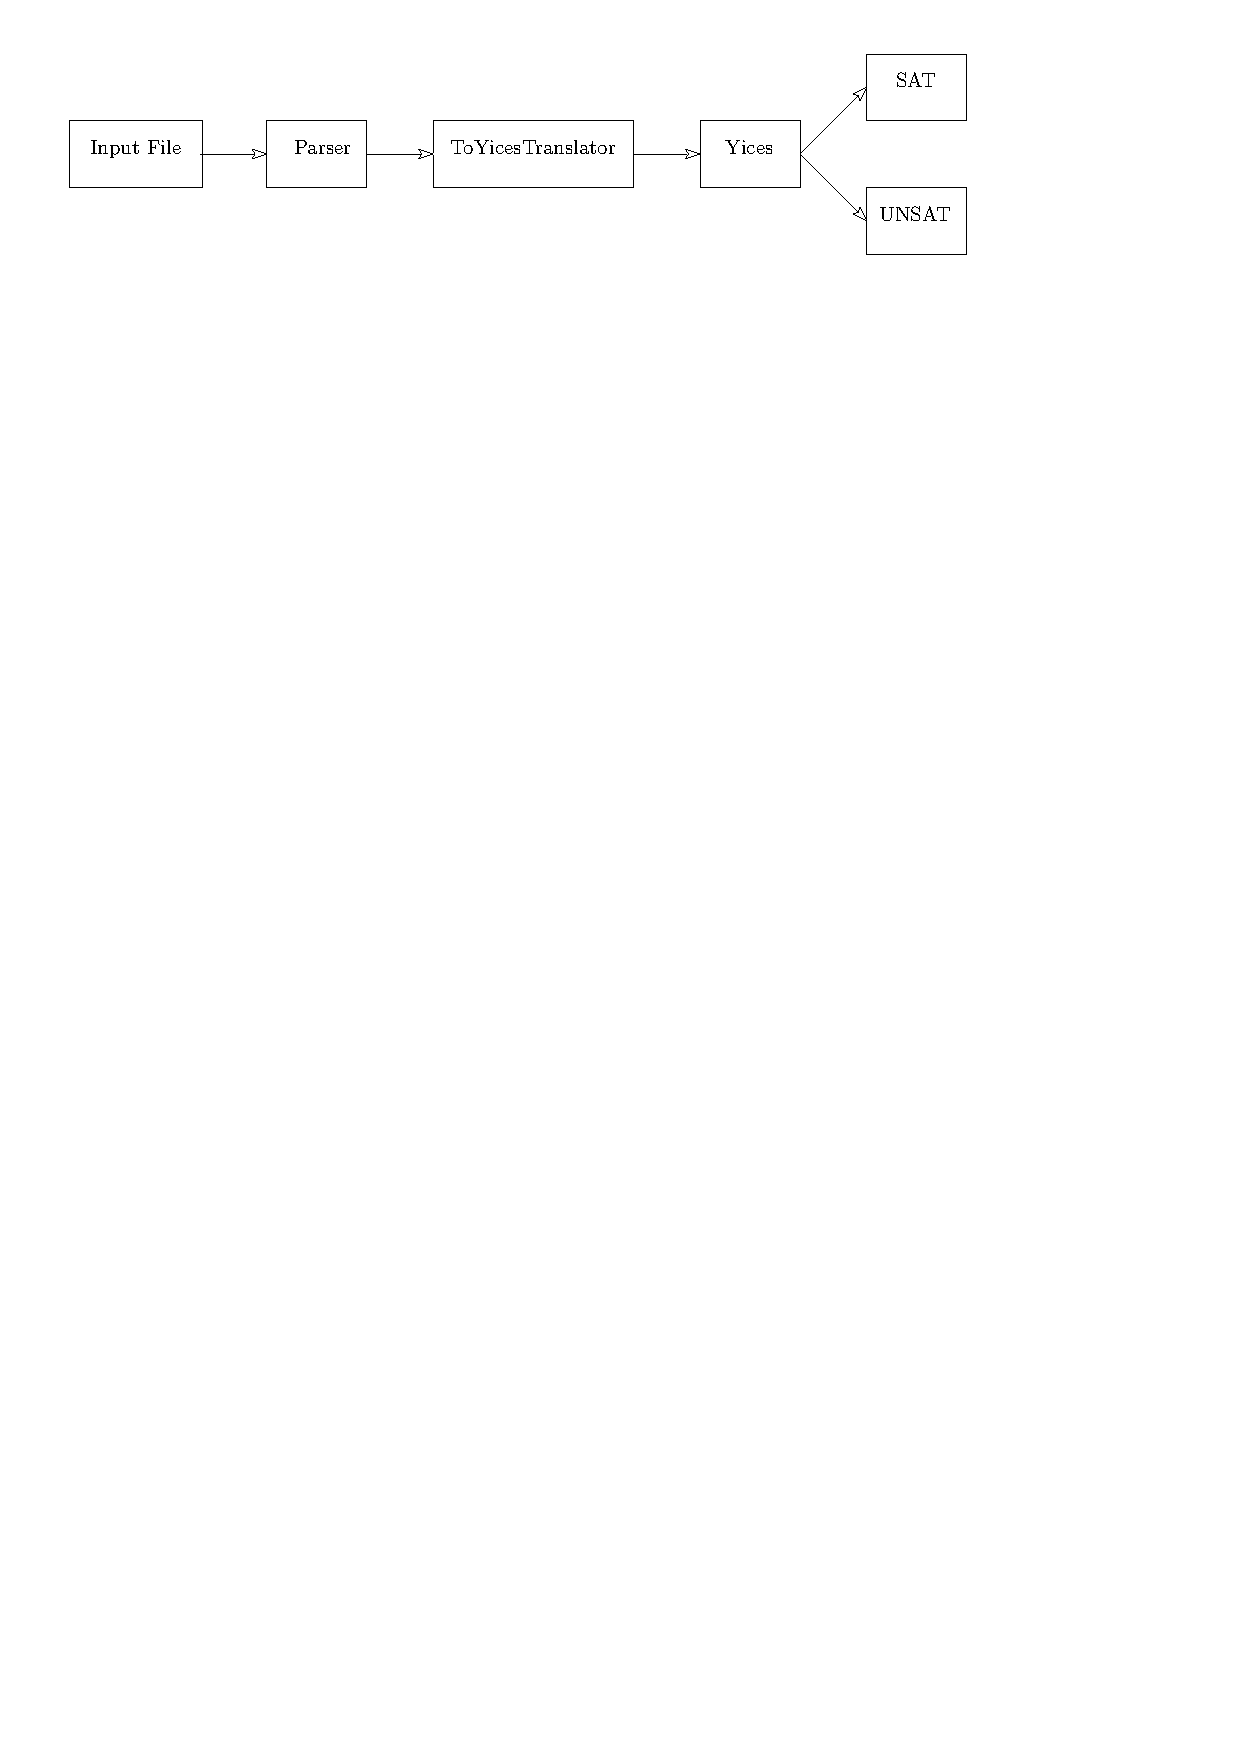
\includegraphics[height=2.5cm, width=\linewidth]{BlockDiagram_horizontal.pdf}
\caption{BlockDiagram of the satisfiability checking engine} \label{fig1}
\end{figure}

\noindent
\[
[0 - 9]+(.[0 - 9]+)? \{ 
    \text{yylval.value = atof(yytext)};
    \text{  return NUMBER};
\}
\]

\noindent
yacc: Yet Another Compiler Compiler is an unix utility that parses a stream
of token generated by lex according to the user specified grammar.Our yacc source 
program has three parts :
  
  \noindent
  declarations\\  
  \%\%\\    
  translation rules\\  
  \%\%\\  
  C routines\\
  
  \noindent
{\bf Declaration part :}\\
  Declaration part can have two section.In the first section delimited by 
  \%{ and \%}. There we included all cpp files and declared global variables.
  \%{\\
  include "eeConstExpr.h"\\
  include "eeNamedExpr.h"\\  
  eeExpr *store;\\
  \%}
    
   \noindent 
  In the next section , we defined a union datatype,tokens and associations.
  \%union\\
  {\\
    char *str;\\
    double value;\\
  }\\

  \noindent
  \%token $<$str$>$ ID\\
  \%token $<$str$>$ KWD

  \noindent
  \%right LE GE
 
 This two sections are optional.
 
 Declaration Section ends with \%\%.
 
 {\bf translation rules part :}
 
 In this section the grammars are specified for the parser.Each rule signifies 
 a grammar and associated with a semantic action.
 
 program: program VarDeclStmt | VarDeclStmt | program asStmt | asStmt;\\
    
 
This section also ends with %%.\\

{\bf C routines :}\\

C subroutines are called from this section.In our code we have called
yyfinalize() routine.\\
   
   

\noindent
{\bf ToYicesTranslator:} After parsing we get a symbol table and a syntax tree.
Using this symbol table ToYicesTranslator generates an output file that can run 
on Yices. Our input specification can have declaration statement, Assert statement 
and Assume statement.This statement can be a mathematical expression containing infix 
notation and not necessarily all expressions be binary. But Yices works on postfix 
binary expression and only recognize assert statement.This tool converts any expression
into a postfix binary expression.

For example : Let us consider a statement assert (a + b + c = 0);\\
              To work on yices, this expression should be written as\\
               
                 (assert( = (+ (+ a b) c) 0))\\
                 
Symbol Table is basically a data structure maintained by the compiler to keep information
about the variables. In our tool, the generated symbol table is used to contain variables 
name and their value.\\

Syntax tree represents an expression in a tree data structure.Each node of a syntax tree 
is either a terminal or a non-terminal or may be a symbol.\\
                 
                 
\begin{figure}[!h]
\centering
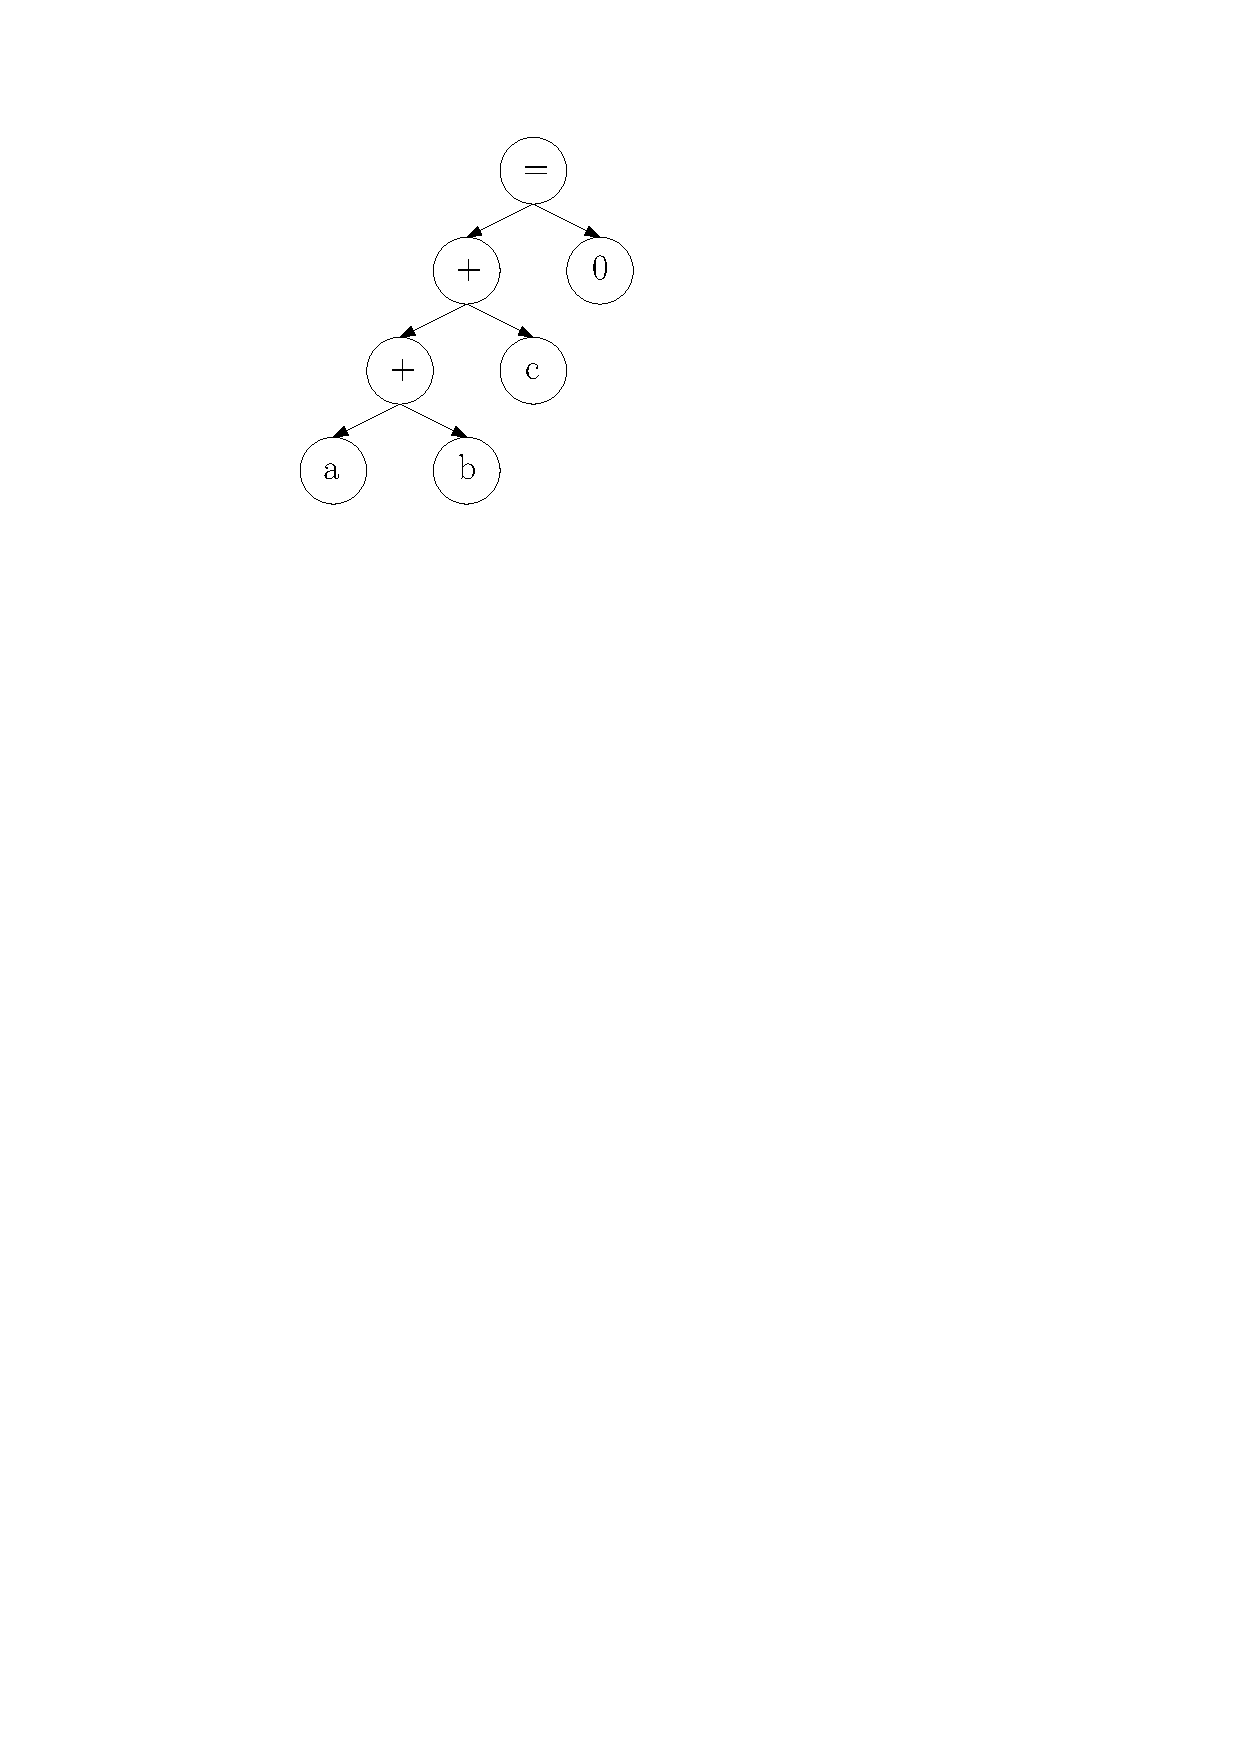
\includegraphics[height=3cm]{syntax_.pdf}
\caption{Syntax tree of the above assert expression} \label{fig1}
\end{figure}



\noindent
{\bf Yices:SMT solver} 

Yices is a Satisfiability Modulo solver to determine the satisfiability of the given assert 
and assume statement. In a yices file the variables are defined, then assert and assume statements
are written on this variables and have .ys extension. Expressions are generally written in postfix
order. Yices tool check whether the given statements are conflicting or not.
For example let us consider two statements\\

x $>$ 5 and x $<$ 4\\

This two conditions cannot occur simultaneously i.e. if x is greater than 5 
then it cannot be smaller than 4. If these two statements are given to Yices
it will give UNSAT output which means the given statements are conflicting.
If instead of the above two statements we had given the following two:\\

x $>$ 5 and y $>$ 4\\

Then Yices would give SAT as output as there was no contradiction between the two
statements. 

\noindent
{\bf Working of our Tool:} The function of ToYicesTranslator is to take 
input of a file containing variable declaration, assert statement, assume 
statement and generate a output file which can run on Yices.The input file
cannot be directly given to Yices as Yices follows a different syntax than
the way these assert and assume statements are written. Hence our Tool acts 
like a bridge between this two. \\

Let us consider a sample input file inFile which contains the following statements:\\

int a, b, c;\\

double f, g;\\

assert ( a + b = 5 );\\

assume ( a $>$ b $>$ c $>$ 6 );\\

assert ( f + g $>$ 10.0 );\\


In the above written file there are two variable declaration statements, two assert
statements and one assume statement. The Input File can have either of assert or 
assume statement or may contain both like the consider File. The variables on
which these assert and assume statements are defined should be declared at the
begining of the file. If assume or assert are defined on an undefined variable 
or a variable is declared more than once then our Tool will generate error specifying
the line number.The output File will have Variable declaration and all assert 
 statements as Yices cannot recognize assume.\\

Now this input file is fed to the parser. Lex specifies the rule and Yacc specifies 
the grammar, at the end of this phase a symbol table is generated which contains each
variable, their names, value and type.  Further more, parser also generates Syntax
Tree, where each expression is represented as a tree where each node holds an element
from the expression. \\

Now using this symbol Table our Tool defines each variable according to Yices format
to their type.  \\

     (define a::int);\\
     
  Using the Syntax tree ToYicesTranslator rearrange the assume or assert expression 
  according to Yices format. \\
  For example,\\
     
    (1)   assert ( a + b = 5);\\
       
   will be converted to:-\\
   
       assert ( = ( a + b ) 5);\\
      
    (2)  assume ( a $>$ b $>$ c $>$ 6 );\\
    
    will be converted to:-\\
    
    \noindent
       assert ( $>$ c 6 );\\
       assert ( $>$ b c );\\
       assert ( $>$ a b );\\
       
At the end of this phase ToYicesTranslator generates the output file
which is compatible with Yices.\\

The output File statements :\\

\noindent
(define a::int)\\
(define b::int)\\
(define c::int)\\
(define f::double)\\
(define g::double)\\
(assert(= (+ a b) 5))\\
(assert($>$ c 6))\\
(assert($>$ b c))\\
(assert($>$ a b))\\
(assert($>$ (+ f g) 10.000000))\\
(check)

At the end of the above file '(check)' is added so that the file can be directly 
fed to Yices Tool without any manual intervention.\\

Yices checks whether the given assertions are conflicting or not. If there
exists at least one case where the conditions are satisfiable then Yices will 
give SAT.If there exist no such case then it says UNSAT.\\

{\small
\begin{thebibliography}{99}

\bibitem{ARM} {\em ARM AMBA Specification Rev 2.0}, http://www.arm.com

\bibitem{das:05} Das, S. et al,
    Formal Methods for Analyzing the
    Completeness of an Assertion Suite against a High-Level Fault model,
    In VLSI Design, 2005.

\bibitem{roadmap} Dasgupta, P., A Roadmap for Formal Property Verification,
        Springer 2006.

\bibitem{lily} Lily, http://www.ist.tugraz.at/staff/jobstmann/lily/

\bibitem{ocp} Open Core Protocol, http://www.ocpip.org 

\end{thebibliography}

\end{document}
